\section{方法} 
\label{sec:proposed}

\begin{figure*}[!tbp]
	\centering
	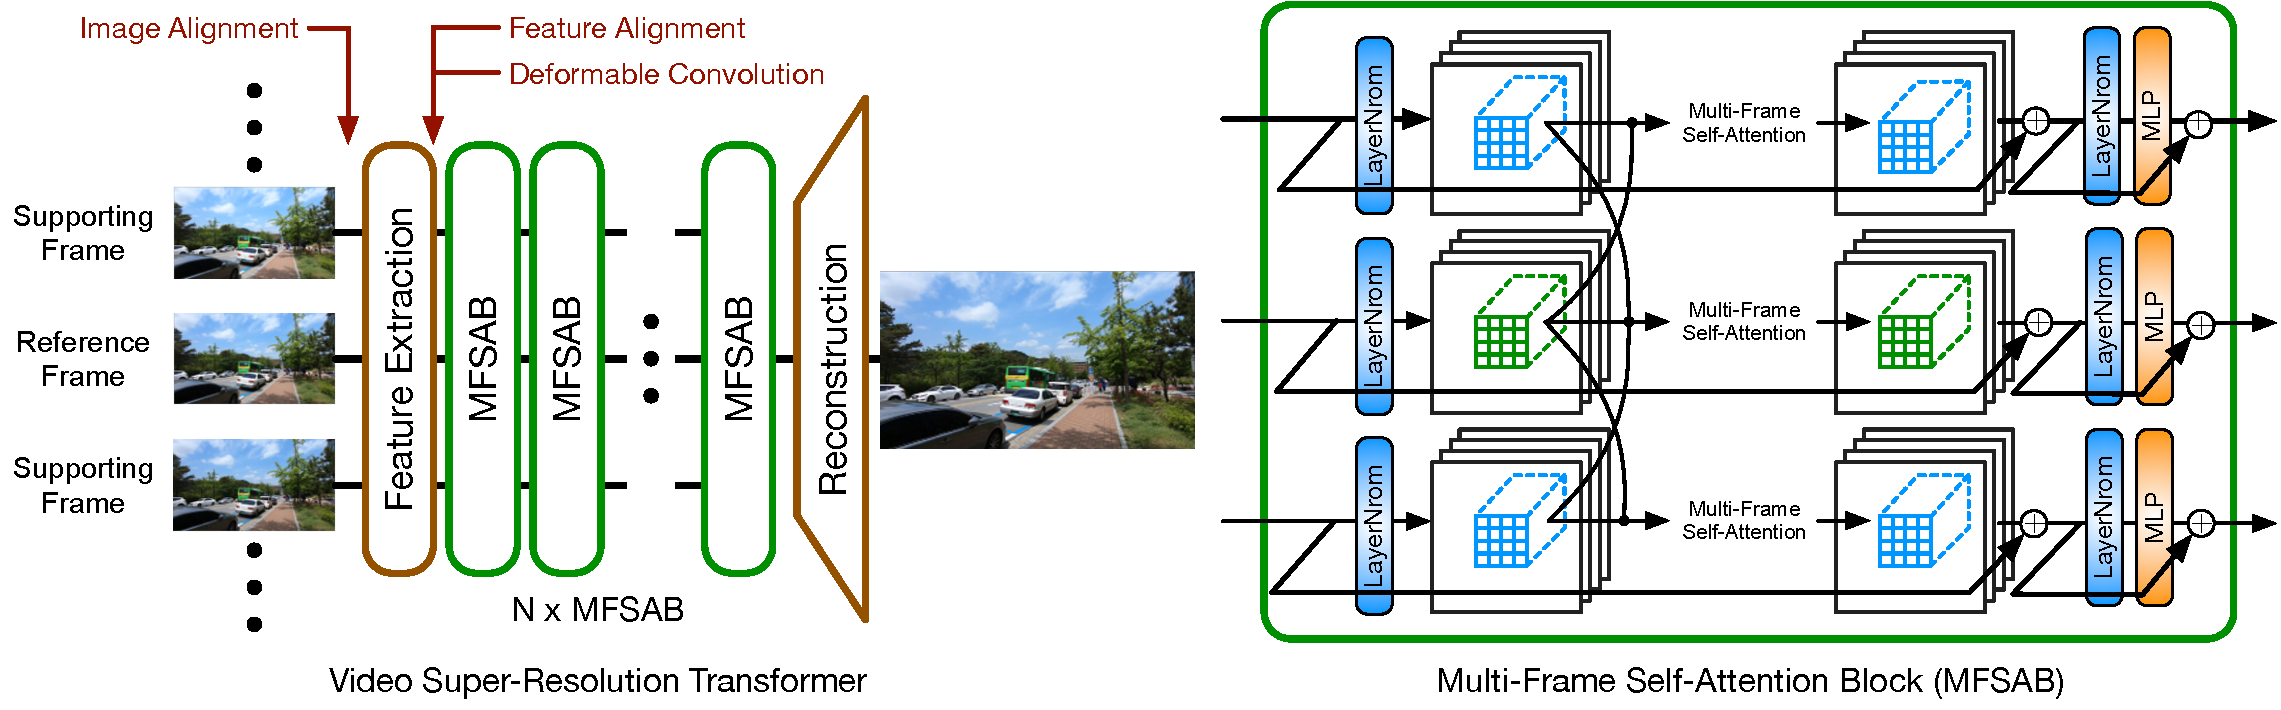
\includegraphics[width=\linewidth]{9.pdf}
	\caption{VSR Transformer 结构示意图}
	\label{fig:fig9}
\end{figure*}

视频超分辨需要 Alignment 是由于 CNN 有非常严格的局部性的归纳偏置而不得不用,但Transformer没有归纳偏置,所以本文提出的第一个思考就是建立一个 VSR 的Transformer 是否仍然需要 Alignment。现有的大部分做法还是延续设计非常复杂的对齐方法,有的时候会占到整个网络近一半的参数。那么自然就会想到如果真的可以不用 alignment,那是用的好还是不用更好呢。

为了研究这两个问题,就需要把这个研究对象给收集起来。使用现有的最基本的图像超分辨或者视频超分辨的Transformer设计来构造了本文的Transformer,如 \textbf{图 \ref{fig:fig9}} 所示,它没有任何特殊的设计。这个模型是基于滑动窗口的,即以三帧作为输入,对中间帧进行超分,前后的这两帧为支持帧(supporting frame),它提供了一些亚像素的信息来支持对中间帧的超分。

Transformer 使用了一个比较通行的标准,即Swin Transformer。Transformer中自注意力的操作会把图像划分成一个一个的局部块。如果不划分局部块而对全局做自注意力的话,在把每一个像素当做一个token的情况下,token数目将会非常多。图像的尺寸增加一倍,token的数量将会增加四倍,其复杂度至少是以 $n^2$ 来增长的。当把图像划分成一个一个的 patch 的时候,即使增大图像的尺寸,其实是patch 的数量在增大,而每一个 patch 里面做的计算仍然是固定数量的像素之间的自注意力操作,其复杂度增加就是线性的。这个 patch 被称为 Attention Window。在这个窗口里面,所有的像素彼此之间有交互,但是窗口和窗口外的像素就没有交互,为了让更多的像素彼此交互,模型会在每一层之间把Attention Window进行位移,称之为 Shift Window。通过这样的方式,就可以让整张图片的任意两个像素可以做一个间接的交互。

本文的模块把 Swin Transformer 从单帧扩展到了一个多帧的情况。例如,原来只有一帧的时候,只是当前 Window $8 \times 8$ 的区域里面 64个像素彼此做自注意力计算。而当把前后帧的像素也纳入进来后,那么同一个位置就是 $3\times 64$(以3帧为例)个像素彼此之间做自注意力计算。

为了研究 Alignment 的影响,还需要对这一模块进行设计。现有的Alignment大致可以分为以下几类:
\begin{enumerate}
	\item 图像对齐是最早最直观的对齐方法。图像对齐依赖于显式计算的帧间光流。根据估计的帧间运动,通过扭曲操作对不同的帧进行对齐。本文使用 SpyNet 来估计光流,并在训练过程中同时对 SpyNet 进行微调,采用 BI 作为重采样方法。
	\item 特征对齐 也可以估计光流,但是是对深度特征进行扭曲操作而不是图像。流估计模块仍然使用SpyNet,在训练时进行优化。除了上图中的二维卷积,此处还额外添加了5个残差块来提取深度特征。
	\item Flow Guide Deformable Convolution 采用可学习的动态可变形卷积进行对齐。几乎所有最先进的VSR网络都使用可变形卷积来进行对齐。本文以 BasicVSR++ 和 VRT 中使用的流引导变形卷积 (FGDC) 对齐作为代表方法。
	\item 无对齐 原始输入直接使用 VSR Transformer 进行处理。
\end{enumerate}


实验涉及到两个主要的Benchmark,一个是REDS,每个视频序列都是比较长的,有100多帧,它的测试集就是REDS 4,有四个100帧左右的测试视频序列。第二个Benchmark的训练集是用Vimeo 90 K,有64,612个训练的视频序列,但是它的每一个视频序列只有七帧。它的测试集有两个数据集,第一个就是Vimeo 90 K的测试集,有7,824 个也是七帧的视频序列,另外一个就是Vid4 测试集。

\begin{figure}[!tbp]
\centering
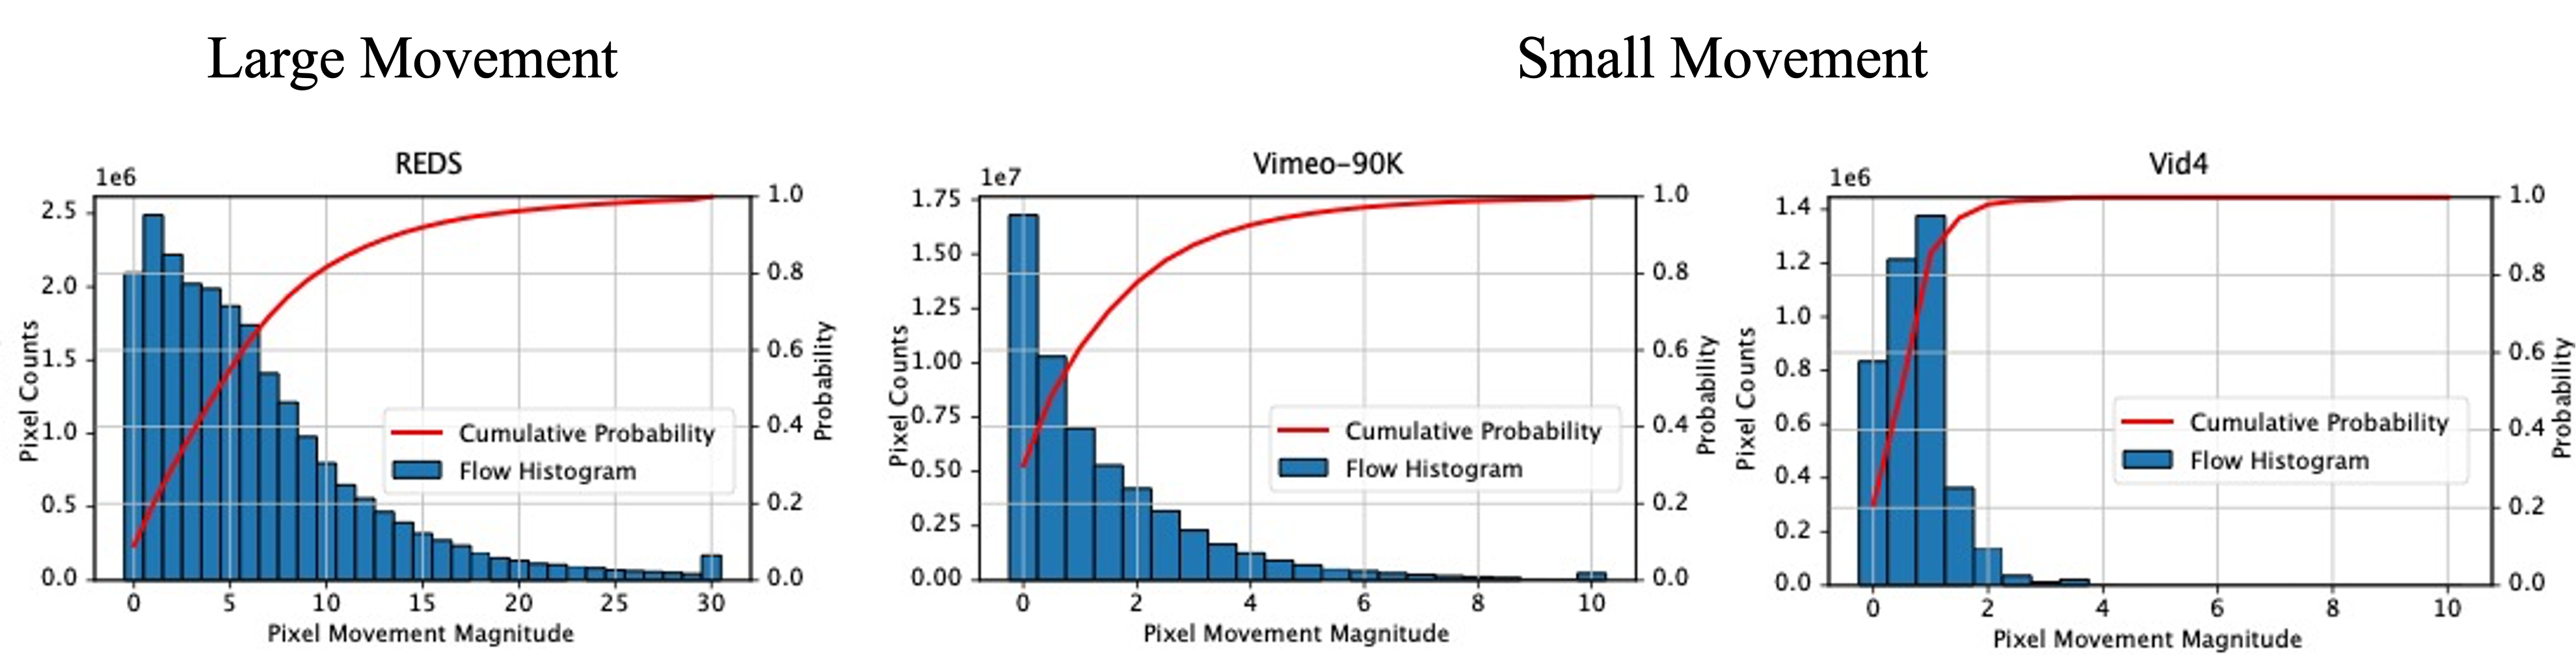
\includegraphics[width=\linewidth]{10.png}	
\caption{不同像素移动条件下,w/o Alignment的VSR Transformer的性能差异}
\label{fig:fig10}
\end{figure}


如 \textbf{图 \ref{fig:fig10}} 所示,可以看到左边的是对 READS 数据集运动情况的统计,在两帧之间,有非常多的物体
是移动了10个、20个甚至30个像素,它的运动来说相对来说非常大。但是右边的这两个数据集,连超过四个像素的运动都非常的少。

回答第一个问题,是不是还要在Video Super-Resolution Transformer里面使用 Alignment的操作呢。

第一个实验使用同一套Transformer的架构构建了两个模型,一个模型使用的是Image Alignment,即先使用光流把图像进行对齐之后再输入到Transformer里面,第二个是不使用Alignment直接输入模型。然后对比不同运动情况像素的 PSNR,如 \textbf{图 \ref{fig:fig11}} 所示,图中大于零的部分代表的是不使用 Alignment会更好,小于零的部分呢是代表使用Alignment会更好。红色的线呢是代表位移是八个像素的这么一条线。在位移小于八个像素的时候,不使用 Alignment明显更好,但是大于八个像素之后,必须使用Alignment才能取得一个更好的成绩。这个八正是Transformer的注意力窗口大小。这个结果表明这个Transformer其实也不是严格意义上的没有归纳偏置,当两个像素同时出现在同一个Window里面时,它可以彼此之间进行直接的交互,不使用Alignment是可以的。但是超出了$8\times 8$的窗口时,它就不能起到这个作用了。而由于运动小于八的像素接近80\%,所以在去看整体的 PSNR 时,会发现不加Alignment会更高。

为了验证它确实是和Attention Window的这个Size是有关的,进一步把Windows Size扩从8扩大到了12,发现它确实在更多的像素上能展示出来不加Alignment就是好。而在换到 Feature Alignment后,当Windows Size是8时,仍然可以获得相同的实验结果。也就是说 Feature Alignment虽然比Image Alignment要更好了。但是他还是没有好到比不加Alignment 还要好的程度。

\begin{figure}[!tbp]
\centering
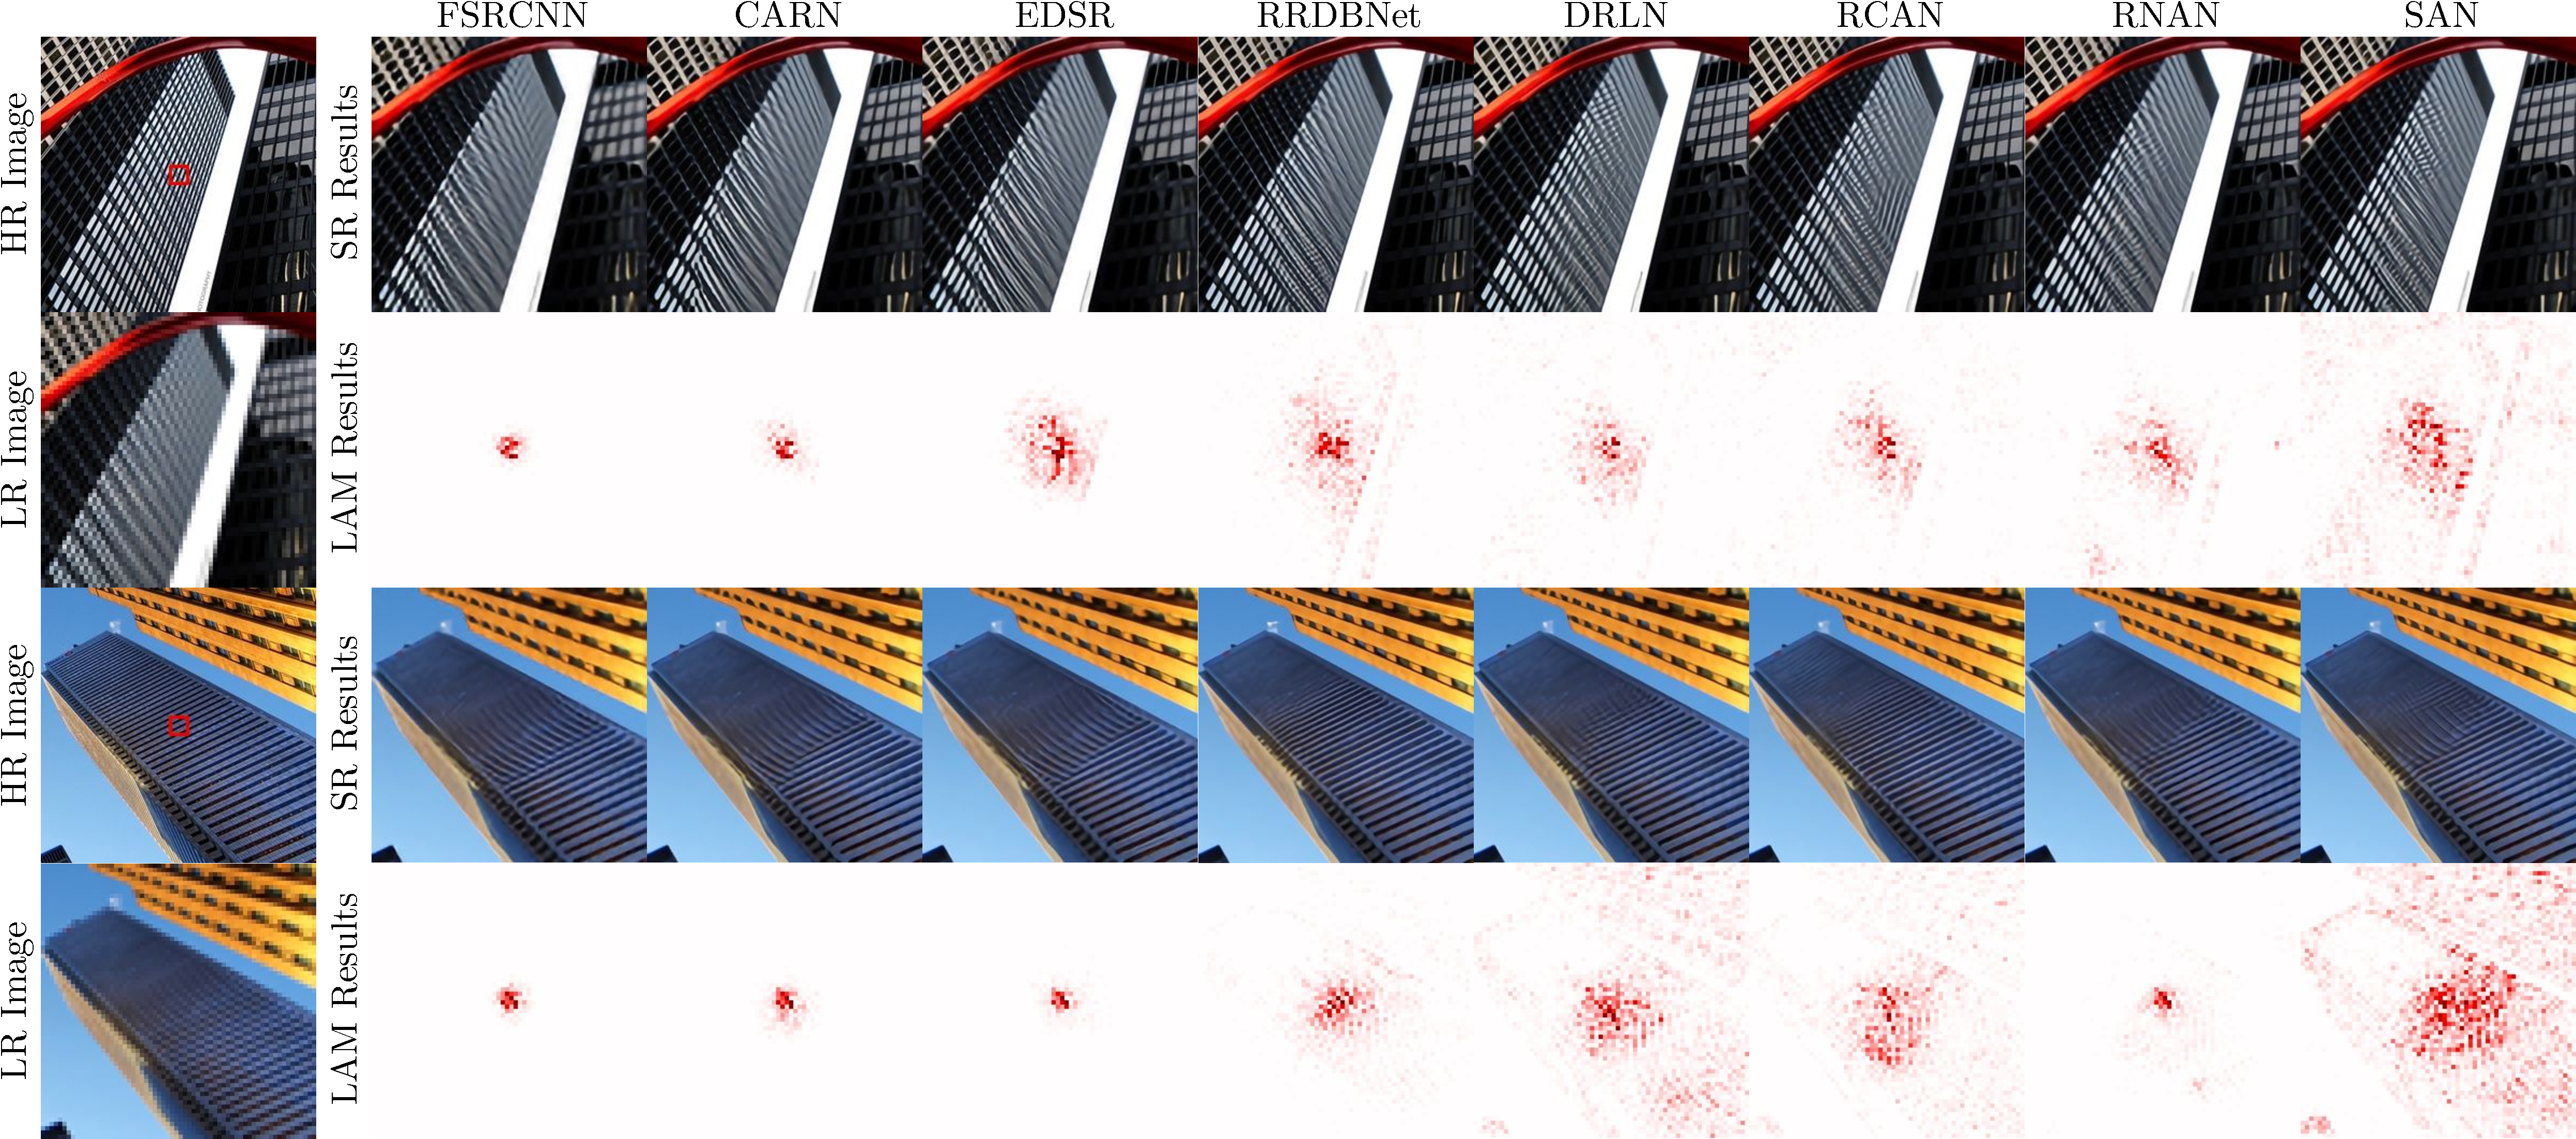
\includegraphics[width=\linewidth]{11.pdf}	
\caption{数据集像素运动分布情况统计}
\label{fig:fig11}
\end{figure}

综上,可以得到三个结论:第一个是 VSR Transformer可以在一定的范围内处理这种不对齐,而且是最好的,这种情况下加上Alignment 反而会损害它的性能;第二是处理的范围是与Transformer里面发挥全局处理的这个范围紧密相关;第三是对于超出这个范围的像素Alignment才是必要的。

\begin{figure*}[!tbp]
	\centering
	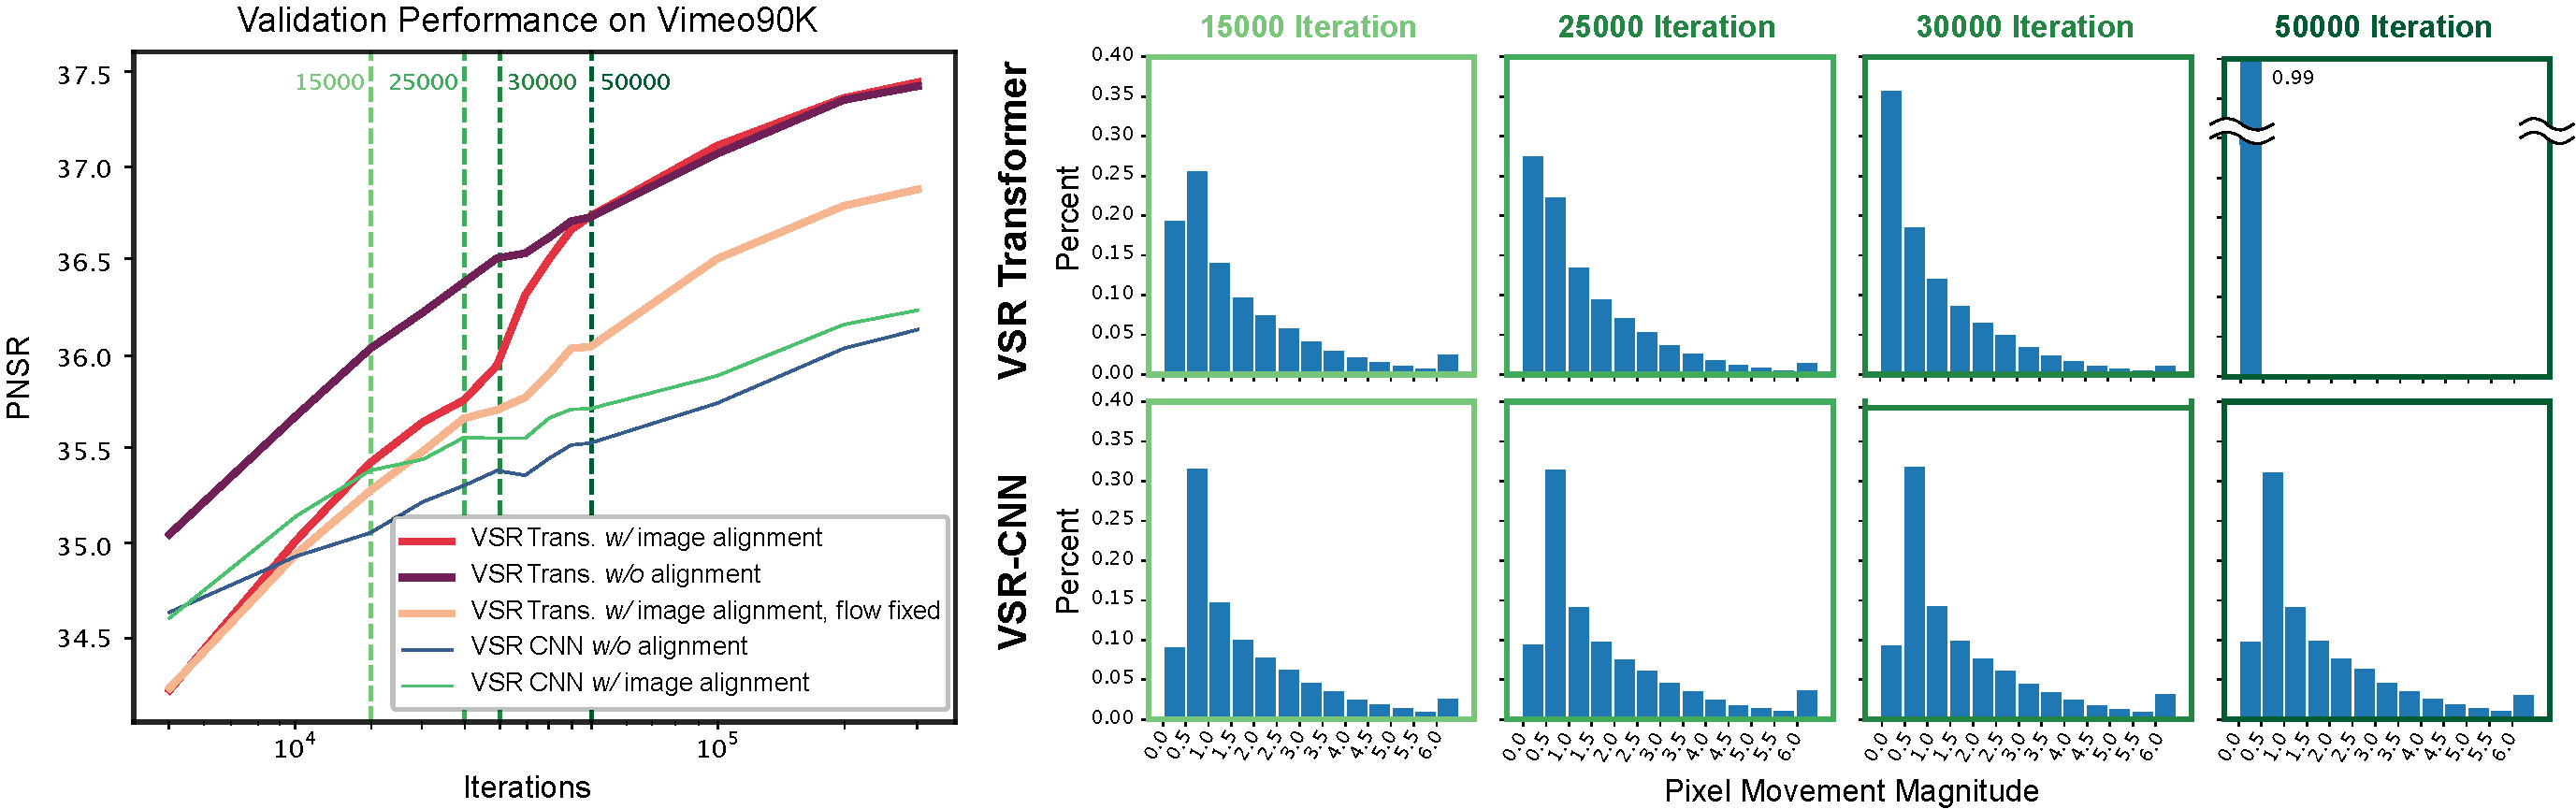
\includegraphics[width=\linewidth]{13.pdf}
	\caption{光流分布示意图}
	\label{fig:fig13}
\end{figure*}

\begin{table*}[!hb]
    \footnotesize
    \caption{Comparison of VSR Transformers with different alignment methods on the REDS4 dataset.}
    \centering
    \label{tab:3-10sliding}
    \vspace{1mm}
    \resizebox{\textwidth}{!}{
    \begin{tabular}{c|cccc|cc|cc|c|c}
        \toprule
        \multirow{2}{*}{\#} & \multicolumn{4}{c|}{Alignment Method} & \multicolumn{2}{c|}{Position} & \multicolumn{2}{c|}{Resampling} & Params. & REDS4\\
        & No Ali. & Img. Ali. & Feat. Ali. & FGDC & Img. & Feat. & BI & NN & (M) & PSNR / SSIM \\
        \midrule
        1 & $\checkmark$ & & & & & & & & 12.9 & 30.92 / 0.8759\\
        2 & & $\checkmark$ & & & $\checkmark$ & & $\checkmark$ & & 12.9 & 30.84 / 0.8752 \\
        3 & & & $\checkmark$ & & & $\checkmark$ & $\checkmark$ & & 14.8 & 31.06 / 0.8792 \\
        4 & & & $\checkmark$ & &  &$\checkmark$ & & $\checkmark$ & 14.8 & 31.11 / 0.8801 \\
        5 & & & & $\checkmark$ & & $\checkmark$ & & & 16.1 & 31.11 / 0.8804 \\
        \bottomrule
    \end{tabular}
    }
\label{tab:tab2}
\end{table*}

接下来再进一步的进行一个可视化或者可解释性的一个研究。为了进一步探究 Transformer 是否真的利用了多帧信息,利用Local Attribution Map高亮出对于处理选定的一小块区域那些非常有用的像素。例如在车牌上圈定一小块像素,用蓝色的线标识出了在中间帧对于这个车牌网络需要关注的位置,红色的区域就是在那一帧当中网络关注到的区域。对于配备了Image Alignment 的 CNN 而言,看到当车牌移开这个蓝色焦点的时候,网络的注意力其实是跟着车牌在走的,注意力红色区域它确实盯在了这个车牌的这个位置。再看不加Alignment的 Transformer,它也有相同的行为,当车牌进行移动的时候,可以发现它的注意力也是从蓝线的右边挪到了蓝线的左边,是跟随着这个物体在走的。也就是说Transformer在没有Alignment的时候他其实是做了一定的对齐的。相反,不加Alignment的CNN,无论车怎么移动,网络的关注点都只会聚焦在原来的位置。

\begin{figure*}[!tbp]
	\centering
	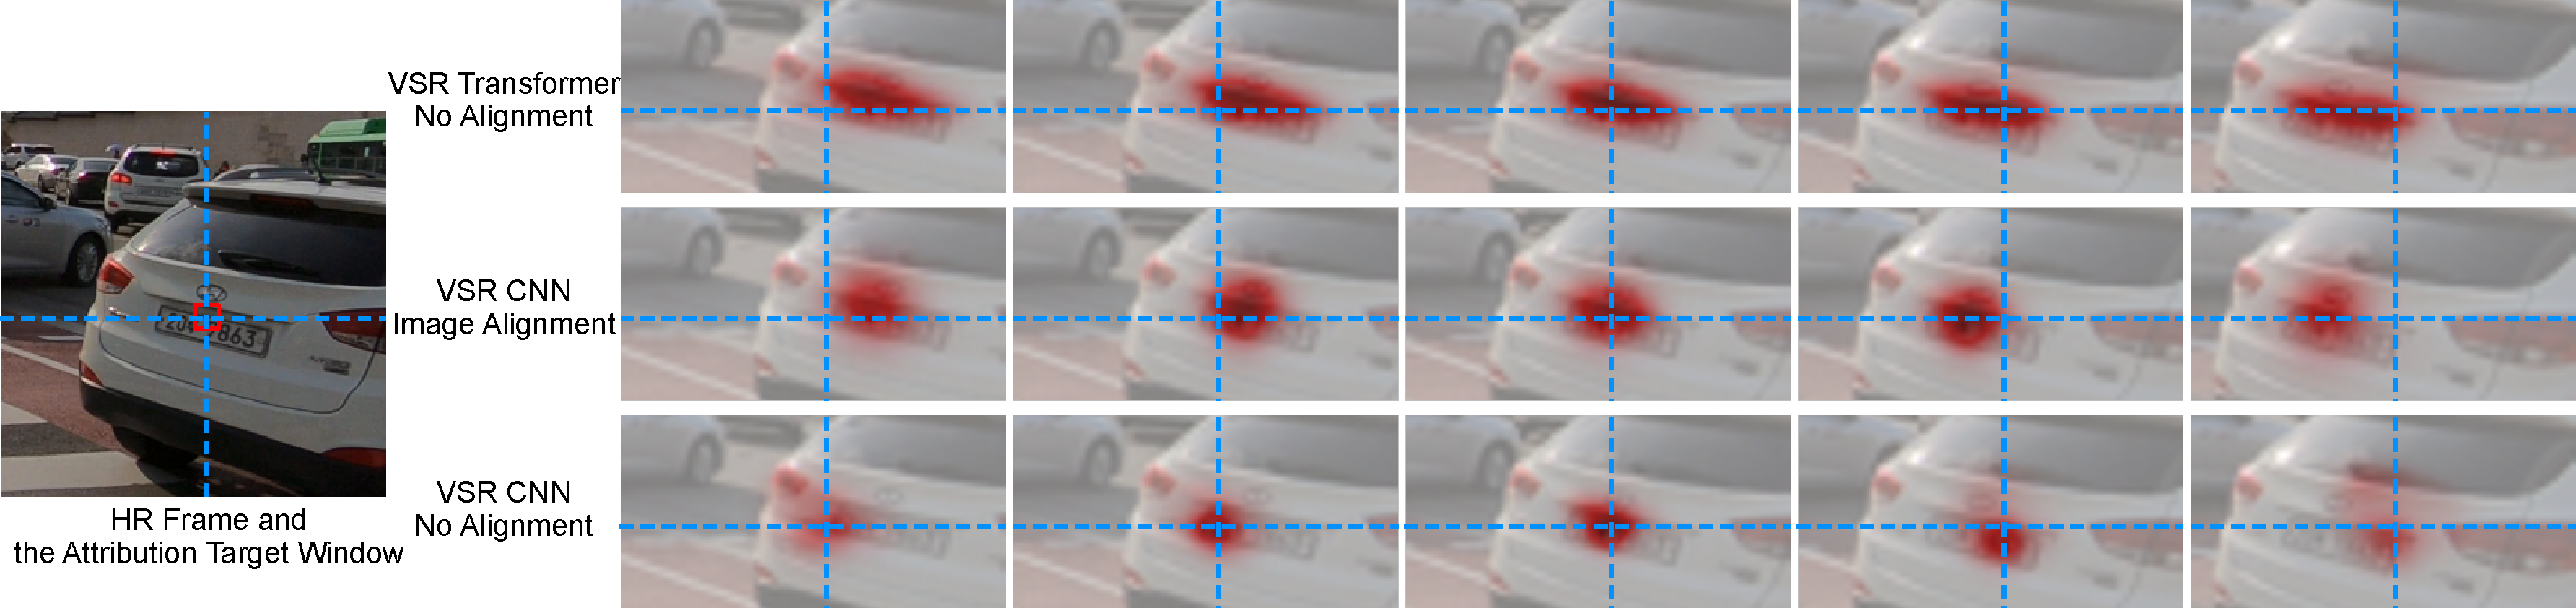
\includegraphics[width=\linewidth]{12.pdf}
	\caption{不同模型的归因结果}
	\label{fig:fig12}
\end{figure*}

\begin{figure*}[!tbp]
	\centering
	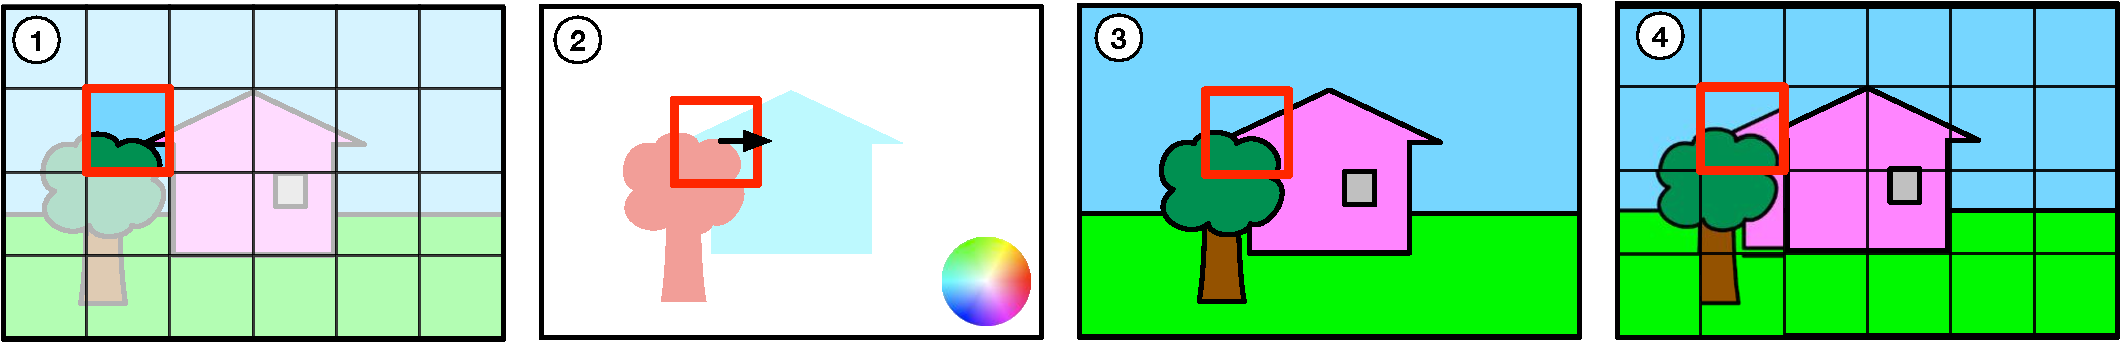
\includegraphics[width=\linewidth]{14.pdf}
	\caption{Patch Alignment: 根据 Transformer 的窗口划分将输入帧划分为 patch,计算每个 patch 的平均运动矢量,在支持帧中找到相应的 patch,并将整个支持 patch 移动到它们相应的位置}
	\label{fig:fig14}
\end{figure*}

对于第二个问题,刚才已经提到了在一定范围内用了alignment 反而会降低它的性能。从实验结果 \textbf{表 \ref{tab:tab1}} 可以看到,就是在 Image Alignment 里,对光流网络进行 Finetune 要比把预测光流的网络固定住要好,因为此时这个网络学习优化的是 VSR 的光流。第二个发现是使用Image Alignment 并 Finetune在Vimeo90K上是37.44,而同样的网络去掉Alignment是37.43非常接近的一个成绩。而在REDS数据集上,后者更是提升了0.13个db。



如 \textbf{图 \ref{fig:fig13}} 所示,最上面的线是是不加 Alignment,红色的线是 Fine Tune 光流网络的线,黄色的线是不Finetune, 可以看到光流固定住之后它的效果肯定就一直和不使用Alignment的保持一定的距离。而红色的线一开始因为初值相同,和 Fix flow的结果是比较接近的,然后随着训练展示出了一点优势,到中间的时候立马追上了不使用Alignment的方法。从预测出来的光流分布可以看到,在25000和30000个iteration的时候分布开始往这个零的方向移动,性能追上来之后,所有的光流都是零。这表明网络认为你虽然给了我这个对齐的模块,但是我发现我不使用你这个对齐模块才是最好的。为了验证说这个东西确实是Transformer特有的,还在CNN上面做了测试,取得了完全不同的结果。


如 \textbf{表 \ref{tab:tab2}} 所示,通过实验发现,造成这个差距的原因主要有两方面,一是预测的光流是有噪声的、不平滑的,这会造成 Warping 的不准确。例如,相邻的两个像素是以不同的光流进行Warping 的,一个往左移动挪了一个像素,另外一个往左移动了0.5个像素,也就是说可能原来这个像素是黑的,另一个像素是白的,Warping 之后移动一个像素位置的像素还是黑色的,移动了0.5个像素位置的像素经过插值不再是白色的,而变成灰色了。在这个过程中,低分辨率的模式中一黑一白经过变成了一黑一灰,即亚像素的信息被改变了,这个改变是一种完全随机的改变,从而减少和伤害了亚像素信息的质量,因而会导致性能的下降。二是在Warping的过程中可能需要重采样,也会引入新的像素值,进而引入新的这个信息损失。在Feature Alignment方法中,简单地把重采样过程从原来广泛使用的双线性采样变成最近邻采样,即Warping前后像素的值是不会改变的,可以看到模型的性能就能达到现在最先进的Flow Guided Deformable Convolution 的一个效果。侧面证明了一部分信息损失是由Eesampling和不准确的光流造成的。

\begin{table}[!ht]
\caption{The Ablation study of Patch Align- ment. We study the effect of different re- sampling methods (BI and NN) and differ- ent alignment positions (image space and feature space).}
    \centering
    \resizebox{0.5\textwidth}{!}{
        \begin{tabular}{c|cc|cc|cc}
        \toprule
        \multirow{2}{*}{Method} & \multicolumn{2}{c|}{Position} & \multicolumn{2}{c|}{Resampling} & \multicolumn{2}{c}{REDS4}\\
         & Img. & Feat. & BI & NN & PSNR & SSIM \\
        \midrule
        \multirow{3}{*}{\shortstack{Patch\\Alignment}} & $\checkmark$ & & & $\checkmark$ & 31.11 & 0.8800 \\
         & & $\checkmark$ & $\checkmark$ & & 31.00 & 0.8781 \\
         & & $\checkmark$ & & $\checkmark$ & 31.17 & 0.8810 \\
        \bottomrule
    \end{tabular}
    }
    \hfill
    % \resizebox{0.38\textwidth}{!}{
    \label{tab:tab3}
\end{table}

至此得到了两个核心的结论:第一个就是Transformer确实可以直接使用没有经过对齐的信息,第二个是现有的这些对齐方法实际上是损失了VSR Transformer 的性能。

而为了设计一个更好的VSR模型,可以简单地扩大Attention Window Size,但这样做会带来巨大的计算开销。因此,作者提出了一个新的对齐方法Patch Alignment。由于光流是不准确的,那么就只用这个大概的这么一个光流,为了不让低分辨率的模式有任何的破坏,直接利用光流均值对整个 Patch进行大概的移动,如 \textbf{图 \ref{fig:fig14}} 所示。

\begin{figure*}[!tbp]
	\centering
	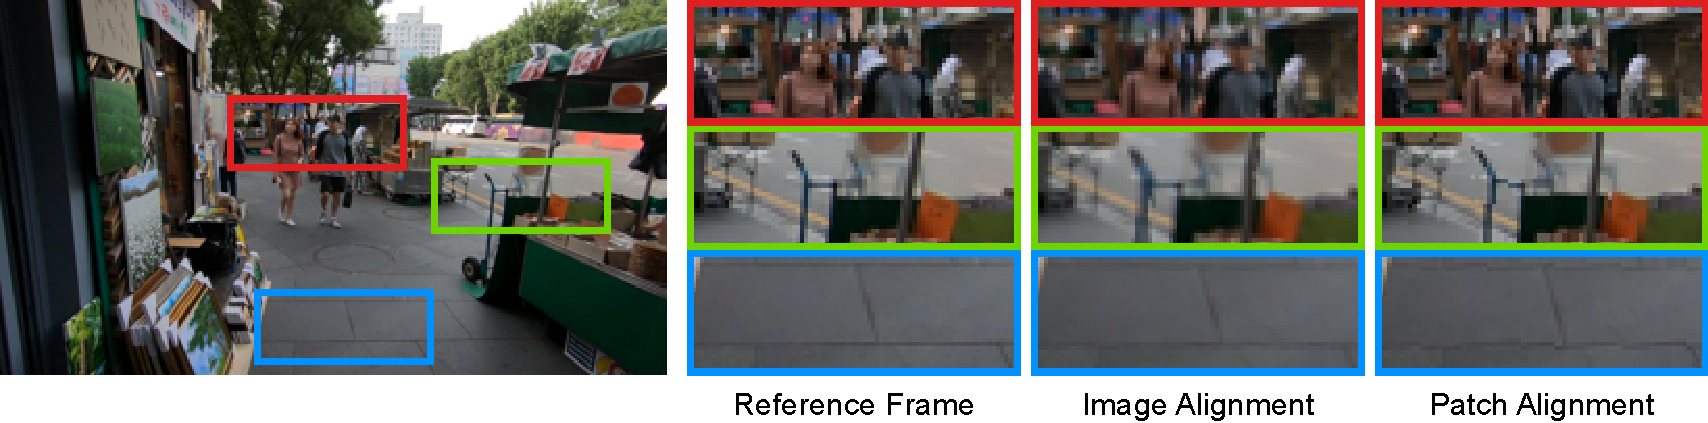
\includegraphics[width=\linewidth]{15.pdf}
	\caption{Image Alignment 和 Patch Alignment可视化结果}
	\label{fig:fig15}
\end{figure*}

再看一下可视化的结果,如 \textbf{图 \ref{fig:fig15}} 所示,第二列是使用Image Alignment的配上双线性插值的重采样,可以看到人脸上非常细小的信息都被模糊掉了,地砖两个像素之间的关系也被破坏掉了。而本文的 Patch Alignment,可以看到这个把手非常的锐利,虽然它有一点点的不对齐,但是这种像素的错位不会带来什么影响,反而只要一个Patch里面的信息不要破坏它就已经是非常好了。
